\chapter[Continuous Integration]{Establishing an efficient workflow for software projects: Continuous Integration}

After having experienced software development in many languages, from desktop programs to mobile applications and web sites, comes a moment when I felt compelled to standardize my software development process. With Matthias' experience, we tried to define The Smiths' workflow more formally, even though they already had something that had been working for a little while.

\medskip

Our main concern was \textbf{continuous integration}. How to properly "synchronize" a team made of many developers, "spread all around the world", in different time zones? Indeed, as I said we were working with a developer from Vietnam. How to make sure there is no bottleneck at any level, during the development? First, let's have a look at the definition.

\medskip

\noindent What is \textbf{continuous integration}? According to Wikipedia, it is:

\begin{quote}
\textit{[...] the practice, in software engineering, of merging all developer working copies to a shared mainline several times a day.}
\end{quote}
But not only. It is much more than this. Let's dive into continuous integration.

\section{Purpose}

Continuous integration is an entire concept that tries to ease software development by making things much easier and flexible. Like agile methodology, it has been getting more and more popular since the beginning of the 2000's. Nowadays, it tends to be widely adopted in any kind of software company.

\subsection{Effortless automation}

Continuous integration is mostly about automation. By this, I mean being able to deploy flawlessly, many times a day. The documentation generation, testing and deploying have to become a commodity. Repetitive tasks are most of the time painful and should be performed by computers.

\subsection{Continuous testing}

\textbf{Every new release has to be tested}. Automatically. Without any human intervention. In a safe and minimal environment, not a human's environment with tons of programs, custom environment variables, outdated dependencies, etc. It is a human job to design the tests but running and validating them is a machine job. This way, the results can be shared with an entire team over automatic emails and archived.

\subsection{Documentation}

Writing documentation is for humans. Generating it is for machines. Again, it is a repetitive task that no one should be assigned. It is a waste of time. Machines can do it instead of us, at the right time, usually when a new release is about to come out. Furthermore, machines do not forget to bump the version numbers.

\subsection{Deploying}

With continuous integration, deploying should be as simple as a \lstinline{git push}. When time has come for deployment, no one should have to use \lstinline{ssh} or \lstinline{rcp}, not even \lstinline{ftp}. \textbf{It is unsafe insofar as it is too much of a risk to let a human get inside a production machine.} A developer has nothing to do in a production machine, as long as all the tests have been passed before pushing to production. All one can do is breaking something. A production machine is meant to be administrated by a sysadmin, no one else. Once it is set up, the only action required by developers is pushing code when it is ready to go live.

\medskip

It is the same story for releases. Packaging and releasing a new version must be a simple task anyone can do, not only the CTO, regardless of the OS, configuration, and so on.

\bigskip
\bigskip

\textbf{That is my point of view about Continuous Integration}, and it is shared by many developers. In fact, continuous integration should simply be regarded as an entire development workflow. It enables a team of developers (or even a single developer) to be more agile. You can easily get rid of god-awful tasks without actually deleting them, just by delegating them to computers. In parallel, it enables developers to improve maintainability and evolvability of the software they produce by adopting the right versioning and bug tracking tools.

\section{Deep diving into continuous integration}

At The Smiths, we identified \textbf{four main components} that we wanted as \textbf{core parts} of \textbf{our Continuous Integration process}:
\begin{itemize}
  \item Semantic versioning
  \item A Git workflow
  \item \href{https://travis-ci.com/}{Travis-ci.org}
  \item Agile methodology
\end{itemize}

\subsection{Semantic versioning}\label{semantic-versioning}

We decided to stick to the very simple rules proposed by \href{http://semver.org/}{semver.org}. Basically, it says that a version number should be something like \textsc{MAJOR.MINOR.PATCH}, where (what follows has been extracted from their website):
\begin{enumerate}
  \item \textsc{MAJOR} version when you make incompatible API changes
  \item \textsc{MINOR} version when you add functionality in a backwards-compatible manner
  \item \textsc{PATCH} version when you make backwards-compatible bug fixes
\end{enumerate}

Sticking to this rule forced us to think more about the logic behind the versions, reshape road maps more precisely, and allowed us to bump our version numbers more cleverly. We applied this to our mobile apps and Titanium widgets, bumping version numbers carefully over time.

\subsection{A successful Git workflow}

This part is clearly the most important, as it is being used every single day by everyone. In general, it is likely the most important aspect about continuous integration, to which we had paid a lot of attention.

\medskip

After some research, we came across a very popular Git workflow, the branching model\footnote{\href{http://nvie.com/posts/a-successful-git-branching-model/}{http://nvie.com/posts/a-successful-git-branching-model/}}. Please refer to the Appendix \ref{appendix-git} for a detailed diagram.

\medskip

Overall, it is the best Git workflow we have ever encountered. \textbf{So we adopted it, with some specificities: we made a few minor changes to that original branching workflow, in order to better suit our needs.} It can be applied to any kind of software project. I also need to mention that we use GitHub, the most famous web-based Git repository hosting service, because it offers some great features, such as Pull requests\footnote{A feature allowing anyone to submit code changes to a project, from a cloned repository, to the original one}, a bug tracker (issues), etc. Moreover, as most of our code has been open sourced (except our clients' core apps), it is not a problem at all. By the way, it also gives us a greater visibility, it is like giving away our widgets to the Titanium community thanks to GitHub.

\subsubsection{Our daily Git workflow at The Smiths}

\begin{itemize}
  \item There is a remote repository called \lstinline{origin}. It is owned by an organization created on GitHub called "TheSmiths", which gathers all of us. Then, every -- new -- developer has to fork this repository into their own private GitHub account. The \lstinline{origin} repository will -- most of the time -- \textbf{only} contains two branches: \lstinline{master} and \lstinline{develop}.
  \begin{itemize}
    \item \lstinline{master}: contains only the stable releases (General Availability). Those are production releases.
    \item \lstinline{develop}: contains only "stable" code with newly developed features. It is the latest cutting-edge release (Release Candidate). It may contains some bugs.
  \end{itemize}
  \item No one is allowed to commit into \lstinline{master} nor into \lstinline{develop} (except for the first commit into \lstinline{master}, then \lstinline{develop} is forked from \lstinline{master}), in either \lstinline{origin} or the forked repositories. Not even locally!
  \item There is one developer responsible for the entire project. Let's call him/her \textsc{Integrator}.
  \item To add a new feature, one of the developers create a local branch called \lstinline{feature-x} from \lstinline{develop} and commit into it. They may eventually push this branch to their own forked repository.
  \item When this feature is fully developed and tested, and ready to go into \lstinline{develop}, the developer creates a Pull request from the forked repository to \lstinline{origin} (from branch \lstinline{feature-x} to \lstinline{develop}). Then, only one person can accept it and merge it: \textsc{Integrator}. Pull requests can also be refused; if so, comment(s) must be added, giving the reason(s) of rejection.
  \item If the Pull request has been accepted, everyone has to update their \lstinline{develop} branch (locally and on their forked repository).
  \item The same applies for hotfixes: anyone can create branches called \lstinline{hotfix-y} and create Pull requests from them.
  \item When time has come for a new release, \textsc{Integrator} merges back \lstinline{develop} into \lstinline{master} and tags it with a release number (according to the Semantic versioning, see subsection \ref{semantic-versioning}). Then, everyone updates their \lstinline{master} branch.
\end{itemize}

I have found out that this workflow works pretty well with any of our projects, might it be an entire app or a mere widget. However, as I said we have made some adjustments to the original workflow found on the Internet, making it a bit simpler to use.

\medskip

\textbf{Issues} are also great features brought by GitHub that allow us to track down bugs and list them. One can assign people to fix an issue, and let others know of its progression thanks to emails or notifications. Issues can also be linked to specific commits which helps a lot when tracking regression bugs.

\medskip

Finally, we also took advantage of \textbf{Milestones}, a GitHub feature, which can be seen as a simplified scheduler, permitting us to create deadlines with goals to reach. It is somehow a list of deadlines with progress bars automatically filled as we would create and merge Pull requests.

\subsection{Travis, the all-in-one tool}

What is \href{https://travis-ci.com/}{Travis-ci.org}? Basically, it is an online service delivered through a website, providing sets of virtual machines started especially for a developer whenever needed. Those machines run some scripts and shut down themselves automatically. Usually, a developer sets up their Travis account to run scripts on every \lstinline{git push} performed on a GitHub repository. However, one can configure Travis to be run with any kind of Git hook\footnote{A particular event, such as \textit{push}, \textit{pull request}, etc}. \textbf{Travis is free} but they also have paid services with much more features (that we did not require).\\
So, how was Travis so helpful for us?

\subsubsection{Most common use cases of Travis}

Well, one can imagine dozens of scenarios. Documentation generated from the source on every new \lstinline{git push} in \lstinline{develop}? Easy. Running a whole set of tests automatically? Easy as well.

\medskip

Let's dream a bit further... One of the most fancy things one can do is \textbf{running a set of tests, bump version numbers in the code and the documentation, compiling the software program and generating the updated documentation, pushing the binaries to Amazon S3\footnote{A file system provider, kind of a hosting solution, by Amazon, very popular, trustful and cheap} and the documentation to GitHub Pages\footnote{\href{https://pages.github.com/}{https://pages.github.com/}}, and making the whole set available to everyone, automatically!} And yes, Travis, can push into specific branches as well. That might be really useful to update web pages automatically (a link to the latest stable release, listed on a download page, for instance).

\medskip

That is definitely the most perfect and automated scenario one could imagine, but that is easily achievable, although it would take quite a long time to set it up.

\bigskip

That 6-month internship did not allow me to do much on Travis. Some of our old Titanium widgets were put on Travis, set up to be compiled on every \lstinline{git push} to make sure nothing was broken. At some point, Matthias (mostly him) and I conducted research about how to best marry Titanium with Travis. In a near future, they will try to tie Travis to every new project (either apps or widgets) to adopt a robuster development workflow.

\subsection{Agile methodology}\label{agile-methodology}

Last but not least, agile methodology. Behind that term that sounds rather complex is a concept pretty simple. In Computer Science, we use the term "Agile Software Development". Wikipedia says:

\begin{quote}
\textit{Agile Software Development is a set of software development methods in which requirements and solutions evolve through collaboration between self-organizing, cross-functional teams. It promotes adaptive planning, evolutionary development, early delivery, continuous improvement, and encourages rapid and flexible response to change.}
\end{quote}

There is also an official \textit{Agile Manifesto} that tries to describe it more precisely, based on twelve principles. \textbf{From that original manifesto have appeared dozens of practices that we refer to as "Agile methods"}. I will not explain them here as it is not the purpose, for more information visit the Wikipedia page\footnote{\href{https://en.wikipedia.org/wiki/Agile_software_development}{https://en.wikipedia.org/wiki/Agile\_software\_development}}.

\medskip

The one we picked is called \textbf{Scrum}. Again, I will not explain it here but will instead expose the workflow we adopted, derived from it. For a better comprehension, I recommend you read the Wikipedia page\footnote{\href{https://en.wikipedia.org/wiki/Scrum_(software_development)}{https://en.wikipedia.org/wiki/Scrum\_(software\_development)}}.

\medskip

We mostly experienced it during our last project, that started in mid-December 2015 and lasted until February 2016. Basically, at the very beginning of the project, Pierre met the client and discussed with them. As a result, he obtained detailed specifications from them. Then, all together, we brainstormed and defined Milestones, which are fundamentally the most important steps to a final product. For instance, from scratch, we aimed at developing a MVP\footnote{\textit{Minimum Viable Product}} (which is a working product, see the picture below), then progressively add features, grouping features under Milestones. As a reminder, "Milestones" is a feature of GitHub. Each Milestone would last a week, tops. In Scrum, Milestones are called \textit{Sprints}.

\medskip

Starting with a MVP is the right way to go. The client is always satisfied as they would get a working copy of the product being-developed, at each stage, continuously getting improved. They would not have to wait for weeks or months before being able to test anything.

\begin{figure}[!h]
   \centering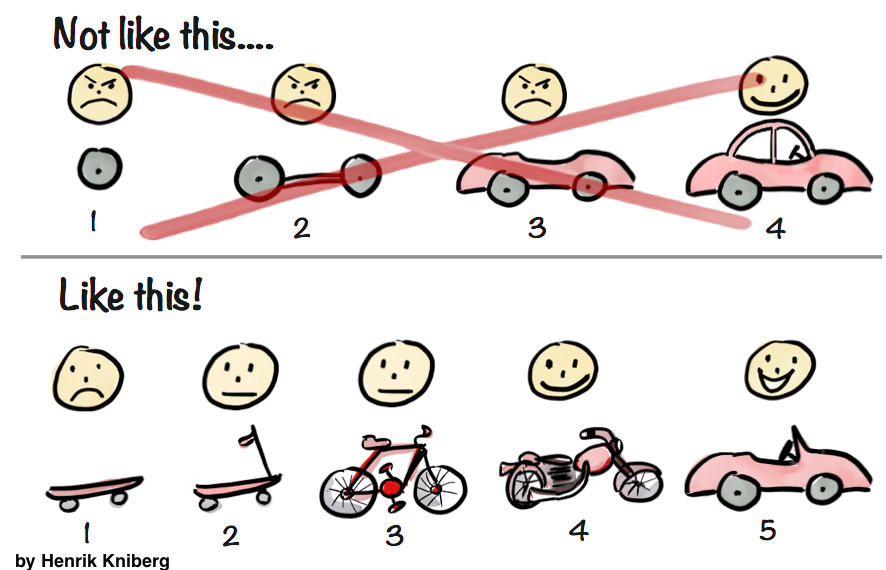
\includegraphics[width=1.00\textwidth]{images/mvp2.png}
   \caption[MVP]{MVP\\Each picture represents a stage in the development process (from left to right), with the client's face above, describing their mood\\Courtesy of \href{https://twitter.com/henrikkniberg/status/685474589539983360}{Henrik Kniberg}}
\end{figure}

Then, each developer would get assigned or choose a few features from the first Milestone until completion. Every morning, we would gather for a 10-minute stand-up meeting, during which everyone would say what they did the previous day and what is left to do, especially regarding the current day. Standing forces us to speak concisely and avoid wasting each other's time, since it is not as comfortable as being sat down.

\medskip

At the end of the Milestone's week, we would merge all the Pull requests resulting from the features, then review all together all the work done, conduct tests and create issues on GitHub to be resolved before starting the next Milestone. Eventually, we would readjust the remaining Milestones when needed.

\medskip

This would go on until completion of the final Milestone, which is supposed to bring all the features originally requested by the client.

\begin{figure}[H]
   \centering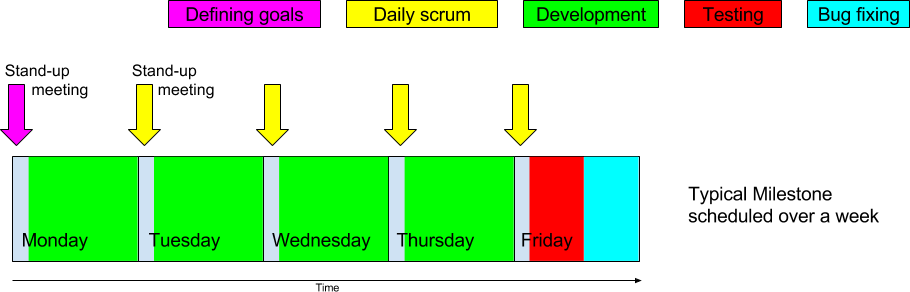
\includegraphics[width=1.00\textwidth]{images/scrum.png}
   \caption[Scrum]{A typical week at The Smiths}
\end{figure}

Sometimes, the part "Bug fixing" would require extra-time. In such a case, we would extend that part onto the next week, only assigning one person, so that the rest of the team could stick strictly to the rule "a Milestone per week". But that rarely happened fortunately.

\subsection{Mix them all}

As a brief conclusion, when thinking back at all the parts of our workflow, one can see that it is an entire whole in which GitHub plays a key-role. Being organized, knowing everyone's role and keeping in mind goals to reach are important as well, just like the tools we decided to go with. Furthermore, being able to release intermediate versions, quickly, allowed us to give constant feedback to the client, which is reassuring.

\medskip

This workflow is surely perfectible, but until now it has proved really efficient. Nevertheless, adapting Titanium apps, not to mention Titanium widgets, to automated tests is still a rather hard thing to do, even though there is an interesting tool developed for UI testing, called Calabash\footnote{\href{https://github.com/appersonlabs/TiCalabash}{https://github.com/appersonlabs/TiCalabash}}.